\documentclass[a4paper,12pt]{article}
\usepackage{times}
\usepackage{hyperref}
\usepackage{xcolor}

\usepackage{geometry}
\geometry{
    a4paper,
    margin=1in,
 }

\usepackage{listings}
\usepackage{xcolor}
\usepackage{multirow}
\usepackage{graphicx}

\definecolor{codegreen}{rgb}{0,0.6,0}
\definecolor{codegray}{rgb}{0.5,0.5,0.5}
\definecolor{codepurple}{rgb}{0.58,0,0.82}
\definecolor{backcolour}{rgb}{0.95,0.95,0.92}

\lstdefinestyle{cppstyle}{
    language=C++,
    backgroundcolor=\color{backcolour},   
    commentstyle=\color{codegreen},
    keywordstyle=\color{magenta},
    numberstyle=\tiny\color{codegray},
    stringstyle=\color{codepurple},
    basicstyle=\ttfamily\footnotesize,
    breakatwhitespace=false,         
    breaklines=true,                 
    captionpos=b,                    
    keepspaces=true,                 
    numbers=left,                    
    numbersep=5pt,                  
    showspaces=false,                
    showstringspaces=false,
    showtabs=false,                  
    tabsize=2
}

\lstdefinestyle{pystyle}{
    language=Python,
    backgroundcolor=\color{backcolour},   
    commentstyle=\color{codegreen},
    keywordstyle=\color{magenta},
    numberstyle=\tiny\color{codegray},
    stringstyle=\color{codepurple},
    basicstyle=\ttfamily\footnotesize,
    breakatwhitespace=false,         
    breaklines=true,                 
    captionpos=b,                    
    keepspaces=true,                 
    numbers=left,                    
    numbersep=5pt,                  
    showspaces=false,                
    showstringspaces=false,
    showtabs=false,                  
    tabsize=2
}

\lstset{style=cppstyle}

\hypersetup{
    colorlinks,
    citecolor=black,
    linkcolor=black,
    urlcolor=black
}

\begin{document}

\begin{titlepage}
    \begin{center}
        \vspace*{1cm}

        \LARGE
        \textbf{Take Home Lab 1}

        \vspace{0.5cm}

        \large
        CS4532 - Concurrent Programming

        \vspace{1.5cm}

        \textbf{190257C - Thamindu Sathruwan\\190332D - Sasitha Kumarasinghe}

        \vfill

        \normalsize
        Department of Computer Science and Engineering\\
        University of Moratuwa\\
        \today

    \end{center}
\end{titlepage}

\tableofcontents
\newpage

\section{Introduction}

This report is about the implementation of concurrent linked lists using mutexes and read-write locks from the \lstinline|pthreads| library. The report will discuss the implementation of linked lists, the configuration of the experiments, the results of the experiments, and a discussion of the results.

\section{Implementation}

The implementation of the linked lists is done in C++ and the code is available in the \lstinline|/src| directory. The code is organized into the following files:

\begin{itemize}
    \itemsep 0em
    \item \textbf{\lstinline|linked_list.h|:} Contains the class interfaces for the linked list implementations.
    \item \textbf{\lstinline|linked_list.cpp|:} Contains the implementation of the linked list classes.
    \item \textbf{\lstinline|threading.h|:} Contains the data structure to pass thread arguments, the thread function, and the function to create and run the threads.
    \item \textbf{\lstinline|threading.cpp|:} Contains the implementation of the above two functions.
\end{itemize}

\subsection{Linked List Interface}

Firstly, an abstract class, \lstinline|LinkedList|, is created as the interface for the linked list implementations. Following the sample code provided, a struct \lstinline|Node| is created as a protected member of the \lstinline|LinkedList| class to represent the nodes of the linked list.

\begin{lstlisting}
class LinkedList
{
public:
    LinkedList() : head(nullptr), length(0) {}

    virtual ~LinkedList()
    {
        Node *curr = head;
        Node *next = nullptr;
        while (curr != nullptr)
        {
            next = curr->next;
            delete curr;
            curr = next;
        }
    }

    void Populate(int n);

    virtual bool Member(int data) = 0;
    virtual bool Insert(int data) = 0;
    virtual bool Remove(int data) = 0;

protected:
    typedef struct Node
    {
        int data;
        Node *next;
    } Node;

    Node *head;
    int length;
};
\end{lstlisting}
\begin{center}
    \textbf{Listing 2.1.1:} \lstinline|LinkedList| class interface
\end{center}

\subsection{Populating the Linked List}

The \lstinline|LinkedList::Populate| method is implemented to populate the linked list with random values. The random seed is taken as the current time and the random number generator is seeded with it.

The linked list is populated as a sorted linked list. For this purpose, a \lstinline|std::set| is used to store the values that are inserted into the linked list. This is done to ensure that the linked list is populated with unique values. Since the \lstinline|std::set| is sorted, the values are inserted into the linked list in sorted order.

Even though the \lstinline|LinkedList::Insert| method is implemented to insert values in the ascending order, it is not used to populate the linked list. The reason is that this function takes a \( O(n) \) time in the worst case. Therefore, to insert \( n \) values, the time complexity would be \( O(n^2) \). The \lstinline|std::set| is implemented using a Red-Black tree which has a worst-case time complexity of \( O(\log n) \). Therefore, the time complexity of inserting \( n \) values into the \lstinline|std::set| is \( O(n \log n) \). This is much better than the \( O(n^2) \) time complexity of inserting values using the \lstinline|LinkedList::Insert| method.

\subsection{Serial Linked List}

The \lstinline|SerialLinkedList| extends the \lstinline|LinkedList| class and implements the serial linked list. The \lstinline|Member|, \lstinline|Insert|, and \lstinline|Remove| methods are implemented to perform the corresponding operations on the linked list. These methods are implemented following the provided code snippets with minimum modifications.

\begin{lstlisting}
class SerialLinkedList : public LinkedList
{
public:
    SerialLinkedList() : LinkedList() {}
    virtual ~SerialLinkedList() {}

    virtual bool Member(int data) override;
    virtual bool Insert(int data) override;
    virtual bool Remove(int data) override;
};
\end{lstlisting}
\begin{center}
    \textbf{Listing 2.3.1:} \lstinline|SerialLinkedList| class interface
\end{center}

\subsection{Concurrent Linked List with Mutexes}

The \lstinline|MutexParallelLinkedList| extends the \lstinline|LinkedList| class and implements the concurrent linked list with mutexes. A new member, \lstinline|pthread_mutex_t mutex|, is added to the class as the mutex for the linked list and initialized in the constructor with \lstinline|pthread_mutex_init| function.

\begin{lstlisting}
    class MutexParallelLinkedList : public SerialLinkedList
    {
    public:
        MutexParallelLinkedList() : SerialLinkedList()
        {
            pthread_mutex_init(&mutex, NULL);
        }
    
        ~MutexParallelLinkedList() {}
    
        bool Member(int data) override;
        bool Insert(int data) override;
        bool Remove(int data) override;
    
    private:
        pthread_mutex_t mutex;
    };
\end{lstlisting}
\begin{center}
    \textbf{Listing 2.4.1:} \lstinline|MutexParallelLinkedList| class interface
\end{center}

Each of the \lstinline|Member|, \lstinline|Insert|, and \lstinline|Remove| methods acquires the mutex before the operation and releases it after the operation is completed. This ensures that only one thread can operate on the linked list at a time. To perform the operation, it calls the same function from the parent \lstinline|SerialLinkedList| class.

\begin{lstlisting}
bool MutexParallelLinkedList::Member(int data)
{
    pthread_mutex_lock(&mutex);
    bool result = SerialLinkedList::Member(data);
    pthread_mutex_unlock(&mutex);
    return result;
}

bool MutexParallelLinkedList::Insert(int data)
{
    pthread_mutex_lock(&mutex);
    bool result = SerialLinkedList::Insert(data);
    pthread_mutex_unlock(&mutex);
    return result;
}

bool MutexParallelLinkedList::Remove(int data)
{
    pthread_mutex_lock(&mutex);
    bool result = SerialLinkedList::Remove(data);
    pthread_mutex_unlock(&mutex);
    return result;
}
\end{lstlisting}
\begin{center}
    \textbf{Listing 2.4.2:} Implementation of \lstinline|Member|, \lstinline|Insert|, and \lstinline|Remove| functions
\end{center}

\subsection{Concurrent Linked List with Read-Write Locks}

The \lstinline|RWLockParallelLinkedList| extends the \lstinline|LinkedList| class and implements the concurrent linked list with read-write locks. A new member, \lstinline|pthread_rwlock_t rwlock|, is added to the class as the read-write lock for the linked list and initialized in the constructor with \lstinline|pthread_rwlock_init| function.

\begin{lstlisting}
class RwLockParallelLinkedList : public SerialLinkedList
{
public:
    RwLockParallelLinkedList() : SerialLinkedList()
    {
        pthread_rwlock_init(&rwlock, NULL);
    }

    ~RwLockParallelLinkedList() {}

    bool Member(int data) override;
    bool Insert(int data) override;
    bool Remove(int data) override;

private:
    pthread_rwlock_t rwlock;
};
\end{lstlisting}
\begin{center}
    \textbf{Listing 2.5.1:} \lstinline|RwLockParallelLinkedList| class interface
\end{center}

The \lstinline|Member| method acquires the read lock before the operation and releases it after the operation is completed. This ensures that multiple threads can perform the \lstinline|Member| operation at the same time but no modification is allowed. The \lstinline|Insert| and \lstinline|Remove| methods acquire the write lock before the operation and release it after the operation is completed. This ensures that only one thread can perform an \lstinline|Insert| or \lstinline|Remove| operation at a time. To perform each operation, it calls the same function from the parent \lstinline|SerialLinkedList| class.

\begin{lstlisting}
bool RwLockParallelLinkedList::Member(int data)
{
    pthread_rwlock_rdlock(&rwlock);
    bool result = SerialLinkedList::Member(data);
    pthread_rwlock_unlock(&rwlock);
    return result;
}

bool RwLockParallelLinkedList::Insert(int data)
{
    pthread_rwlock_wrlock(&rwlock);
    bool result = SerialLinkedList::Insert(data);
    pthread_rwlock_unlock(&rwlock);
    return result;
}

bool RwLockParallelLinkedList::Remove(int data)
{
    pthread_rwlock_wrlock(&rwlock);
    bool result = SerialLinkedList::Remove(data);
    pthread_rwlock_unlock(&rwlock);
    return result;
}
\end{lstlisting}
\begin{center}
    \textbf{Listing 2.5.2:} Implementation of \lstinline|Member|, \lstinline|Insert|, and \lstinline|Remove| functions
\end{center}

\subsection{Threading}

The implementation of threading is done in the \lstinline|threading.h| and \lstinline|threading.cpp| files. The \lstinline|threading.h| file contains the \lstinline|ThreadArgs| struct to pass the arguments to the thread function. It also contains the declaration of the thread function, \lstinline|thread_func|, and the \lstinline|run_threads| function which creates the threads and runs them.

\begin{lstlisting}
typedef struct ThreadArgs
{
    LinkedList *list;
    int m;
    double mMember;
    double mInsert;
    double mDelete;
    int threadCnt;
    unsigned long tid;
} ThreadArgs;

void *thread_func(void *arg);
long run_threads(int threadCnt, LinkedList *list,
                    int m, double mMember, double mInsert, double mDelete);
\end{lstlisting}
\begin{center}
    \textbf{Listing 2.6.1:} \lstinline|threading.h| file
\end{center}

The implementation of the above two functions is done in the \lstinline|threading.cpp| file. Instead of using global variables to the required parameters, a pointer to the corresponding \lstinline|ThreadArgs|struct is passed as the argument to the thread function. The thread function will perform \( (m \times mMember)\ /\ threadCnt \) number of \lstinline|Member| operations, \( (m \times mInsert)\ /\ threadCnt \) number of \lstinline|Insert| operations, and \( (m \times mDelete)\ /\ threadCnt \) number of \lstinline|Remove| operations with random values. The \lstinline|run_threads| function creates the threads and waits for them to complete. It also calculates the total time taken by the threads to complete the operations.

\section{Sample Size Calculation}

To get the performance results within the required confidence interval and margin of error,
the sample size should be calculated. The sample size is calculated using the following formula:

\[
    n = \frac{z^2 \times \hat{p} \times (1 - \hat{p})}{e^2}
\]

Where \( z \) is the z-score, \( \hat{p} \) is the population proportion, and \( e \) is the margin of error.
We use following python function to calculate the sample size. We passed the confidence level as 0.95,
population proportion as 0.5, and margin of error as 0.05 to the function.

\lstset{style=pystyle}

\begin{lstlisting}
def getSampleSize(confidence_level, population_propotion, error):
    z_score = stats.norm.ppf((1 + confidence_level) / 2)
    return int(round((z_score ** 2) * population_propotion 
        * (1 - population_propotion) / (error ** 2)))
\end{lstlisting}

The calculated sample size is 384. Therefore, we ran the experiments 384 times to get the performance
results within the required confidence interval and margin of error.

\section{Specifications of the Running Computer}

The experiments were run on a computer with the following specifications:

\begin{itemize}
    \itemsep 0em
    \item \textbf{Processor:} Intel(R) Core(TM) i7-8550U CPU @ 1.80GHz   1.99 GHz
    \item \textbf{RAM:} 16GB DDR4
    \item \textbf{System Type:} 64-bit Operating System, x64-based processor
    \item \textbf{OS:} Ubuntu 20.04 LTS
    \item \textbf{WSL Version:} Windows Subsystem for Linux 2 (WSL2) is used to run Ubuntu
    \item \textbf{Physical Cores:} 4
    \item \textbf{Logical Cores:} 8
\end{itemize}

\section{Results}

These are the mean and the standard deviation of the execution times (microseconds) of the
\lstinline|Member|, \lstinline|Insert|, and \lstinline|Remove| operations of
the serial linked list, concurrent linked list with mutexes, and concurrent
linked list with read-write locks.

\subsection{Case 1}

n=1000, m=10000, m\textsubscript{Member}=0.99, m\textsubscript{Insert}=0.005, m\textsubscript{Delete}=0.005

\begin{table}[h]
    \small
    \begin{tabular}{|l|llllllll|}
        \hline
        \multicolumn{1}{|c|}{\multirow{3}{*}{\textbf{\begin{tabular}[c]{@{}c@{}}Implemen\\ -tation\end{tabular}}}} & \multicolumn{8}{c|}{\textbf{No of threads}}                                                                                                                                                                                                                                                                         \\ \cline{2-9}
        \multicolumn{1}{|c|}{}                                                                                     & \multicolumn{2}{c|}{\textbf{1}}             & \multicolumn{2}{c|}{\textbf{2}}   & \multicolumn{2}{c|}{\textbf{4}}       & \multicolumn{2}{c|}{\textbf{8}}                                                                                                                                                           \\ \cline{2-9}
        \multicolumn{1}{|c|}{}                                                                                     & \multicolumn{1}{c|}{\textbf{Average}}       & \multicolumn{1}{c|}{\textbf{Std}} & \multicolumn{1}{c|}{\textbf{Average}} & \multicolumn{1}{c|}{\textbf{Std}} & \multicolumn{1}{c|}{\textbf{Average}} & \multicolumn{1}{c|}{\textbf{Std}} & \multicolumn{1}{c|}{\textbf{Average}} & \multicolumn{1}{c|}{\textbf{Std}} \\ \hline
        Serial                                                                                                     & \multicolumn{1}{c|}{14368.44}               & \multicolumn{1}{c|}{857.82}       & \multicolumn{1}{c|}{-}                & \multicolumn{1}{c|}{-}            & \multicolumn{1}{c|}{-}                & \multicolumn{1}{c|}{-}            & \multicolumn{1}{c|}{-}                & \multicolumn{1}{c|}{-}            \\ \hline
        \begin{tabular}[c]{@{}l@{}}One mutex \\ for entire list\end{tabular}                                       & \multicolumn{1}{c|}{15326.01}               & \multicolumn{1}{c|}{2422.30}      & \multicolumn{1}{c|}{33999.43}         & \multicolumn{1}{c|}{2750.07}      & \multicolumn{1}{c|}{37289.85}         & \multicolumn{1}{c|}{8222.74}      & \multicolumn{1}{c|}{47572.92}         & \multicolumn{1}{c|}{4162.54}      \\ \hline
        \begin{tabular}[c]{@{}l@{}}Read-Write \\ lock\end{tabular}                                                 & \multicolumn{1}{c|}{14563.0}                & \multicolumn{1}{c|}{1128.00}      & \multicolumn{1}{c|}{12125.18}         & \multicolumn{1}{c|}{1668.12}      & \multicolumn{1}{c|}{9752.32}          & \multicolumn{1}{c|}{2223.47}      & \multicolumn{1}{c|}{6828.53}          & \multicolumn{1}{c|}{2747.13}      \\ \hline
    \end{tabular}
\end{table}

Figure \ref{fig:case1} shows the average execution time plot for case 1.

\begin{figure}[h]
    \centering
    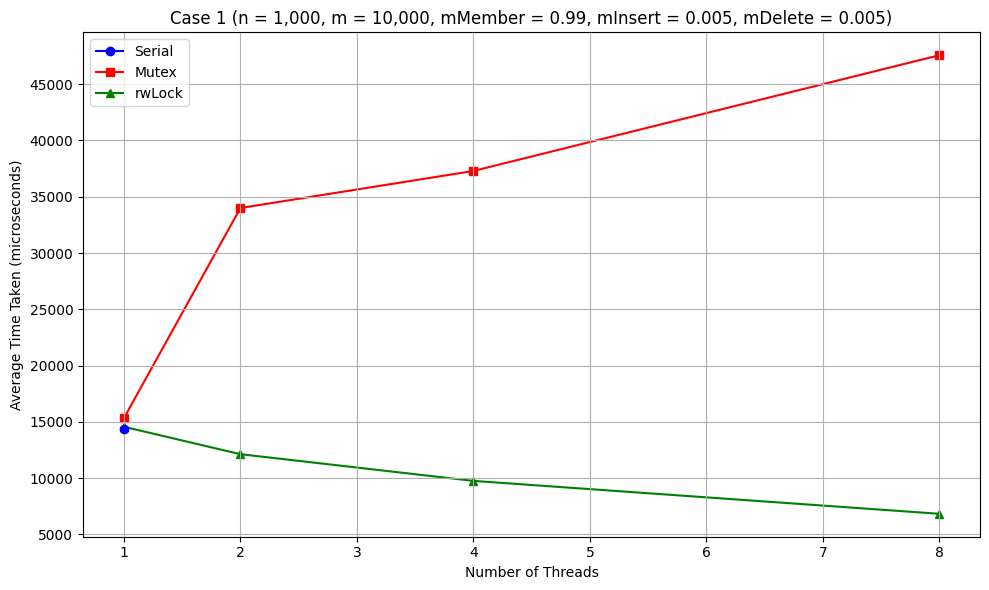
\includegraphics[width=0.9\textwidth]{images/case1.png}
    \caption{Average execution time plot for case 1}
    \label{fig:case1}
\end{figure}

\subsection{Case 2}

n=1000, m=10000, m\textsubscript{Member}=0.90, m\textsubscript{Insert}=0.05, m\textsubscript{Delete}=0.05

\begin{table}[h]
    \small
    \begin{tabular}{|l|llllllll|}
        \hline
        \multicolumn{1}{|c|}{\multirow{3}{*}{\textbf{\begin{tabular}[c]{@{}c@{}}Implemen\\ -tation\end{tabular}}}} & \multicolumn{8}{c|}{\textbf{No of threads}}                                                                                                                                                                                                                                                                         \\ \cline{2-9}
        \multicolumn{1}{|c|}{}                                                                                     & \multicolumn{2}{c|}{\textbf{1}}             & \multicolumn{2}{c|}{\textbf{2}}   & \multicolumn{2}{c|}{\textbf{4}}       & \multicolumn{2}{c|}{\textbf{8}}                                                                                                                                                           \\ \cline{2-9}
        \multicolumn{1}{|c|}{}                                                                                     & \multicolumn{1}{c|}{\textbf{Average}}       & \multicolumn{1}{c|}{\textbf{Std}} & \multicolumn{1}{c|}{\textbf{Average}} & \multicolumn{1}{c|}{\textbf{Std}} & \multicolumn{1}{c|}{\textbf{Average}} & \multicolumn{1}{c|}{\textbf{Std}} & \multicolumn{1}{c|}{\textbf{Average}} & \multicolumn{1}{c|}{\textbf{Std}} \\ \hline
        Serial                                                                                                     & \multicolumn{1}{c|}{16559.35}               & \multicolumn{1}{c|}{2633.58}      & \multicolumn{1}{c|}{-}                & \multicolumn{1}{c|}{-}            & \multicolumn{1}{c|}{-}                & \multicolumn{1}{c|}{-}            & \multicolumn{1}{c|}{-}                & \multicolumn{1}{c|}{-}            \\ \hline
        \begin{tabular}[c]{@{}l@{}}One mutex \\ for entire list\end{tabular}                                       & \multicolumn{1}{c|}{17042.13}               & \multicolumn{1}{c|}{2226.58}      & \multicolumn{1}{c|}{39230.61}         & \multicolumn{1}{c|}{6043.93}      & \multicolumn{1}{c|}{46875.51}         & \multicolumn{1}{c|}{8381.03}      & \multicolumn{1}{c|}{53189.61}         & \multicolumn{1}{c|}{6066.44}      \\ \hline
        \begin{tabular}[c]{@{}l@{}}Read-Write \\ lock\end{tabular}                                                 & \multicolumn{1}{c|}{18679.82}               & \multicolumn{1}{c|}{4403.54}      & \multicolumn{1}{c|}{23186.73}         & \multicolumn{1}{c|}{10084.84}     & \multicolumn{1}{c|}{13628.77}         & \multicolumn{1}{c|}{2173.77}      & \multicolumn{1}{c|}{11339.61}         & \multicolumn{1}{c|}{2384.95}      \\ \hline
    \end{tabular}
\end{table}

Figure \ref{fig:case2} shows the average execution time plot for case 2.

\begin{figure}[h]
    \centering
    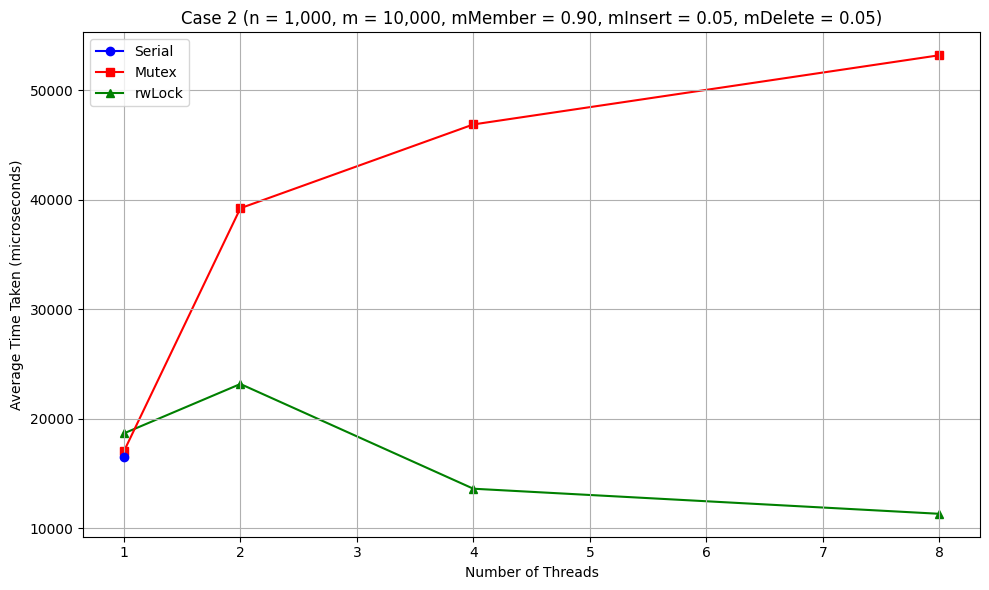
\includegraphics[width=0.9\textwidth]{images/case2.png}
    \caption{Average execution time plot for case 2}
    \label{fig:case2}
\end{figure}

\subsection{Case 3}

n=1000, m=10000, m\textsubscript{Member}=0.5, m\textsubscript{Insert}=0.25, m\textsubscript{Delete}=0.25

\begin{table}[h]
    \small
    \begin{tabular}{|l|llllllll|}
        \hline
        \multicolumn{1}{|c|}{\multirow{3}{*}{\textbf{\begin{tabular}[c]{@{}c@{}}Implemen\\ -tation\end{tabular}}}} & \multicolumn{8}{c|}{\textbf{No of threads}}                                                                                                                                                                                                                                                                         \\ \cline{2-9}
        \multicolumn{1}{|c|}{}                                                                                     & \multicolumn{2}{c|}{\textbf{1}}             & \multicolumn{2}{c|}{\textbf{2}}   & \multicolumn{2}{c|}{\textbf{4}}       & \multicolumn{2}{c|}{\textbf{8}}                                                                                                                                                           \\ \cline{2-9}
        \multicolumn{1}{|c|}{}                                                                                     & \multicolumn{1}{c|}{\textbf{Average}}       & \multicolumn{1}{c|}{\textbf{Std}} & \multicolumn{1}{c|}{\textbf{Average}} & \multicolumn{1}{c|}{\textbf{Std}} & \multicolumn{1}{c|}{\textbf{Average}} & \multicolumn{1}{c|}{\textbf{Std}} & \multicolumn{1}{c|}{\textbf{Average}} & \multicolumn{1}{c|}{\textbf{Std}} \\ \hline
        Serial                                                                                                     & \multicolumn{1}{c|}{24701.33}               & \multicolumn{1}{c|}{4609.62}      & \multicolumn{1}{c|}{-}                & \multicolumn{1}{c|}{-}            & \multicolumn{1}{c|}{-}                & \multicolumn{1}{c|}{-}            & \multicolumn{1}{c|}{-}                & \multicolumn{1}{c|}{-}            \\ \hline
        \begin{tabular}[c]{@{}l@{}}One mutex \\ for entire list\end{tabular}                                       & \multicolumn{1}{c|}{22068.34}               & \multicolumn{1}{c|}{1568.51}      & \multicolumn{1}{c|}{50801.73}         & \multicolumn{1}{c|}{7032.42}      & \multicolumn{1}{c|}{69534.08}         & \multicolumn{1}{c|}{16038.64}     & \multicolumn{1}{c|}{95056.90}         & \multicolumn{1}{c|}{17094.91}     \\ \hline
        \begin{tabular}[c]{@{}l@{}}Read-Write \\ lock\end{tabular}                                                 & \multicolumn{1}{c|}{22973.35}               & \multicolumn{1}{c|}{2311.93}      & \multicolumn{1}{c|}{52427.07}         & \multicolumn{1}{c|}{16754.70}     & \multicolumn{1}{c|}{54487.90}         & \multicolumn{1}{c|}{11847.46}     & \multicolumn{1}{c|}{63159.63}         & \multicolumn{1}{c|}{8815.97}      \\ \hline
    \end{tabular}
\end{table}

Figure \ref{fig:case3} shows the average execution time plot for case 3.

\begin{figure}[h]
    \centering
    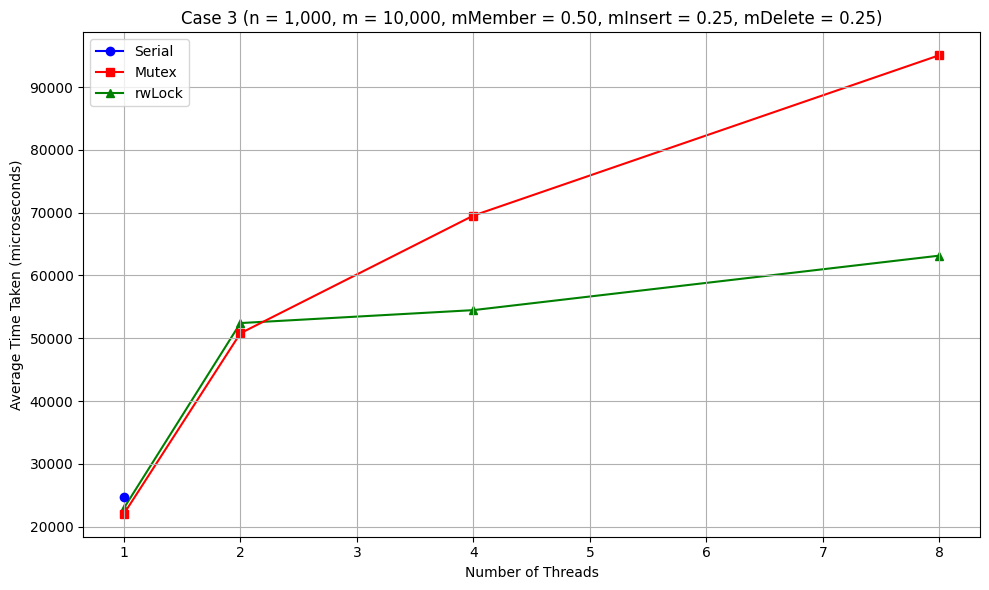
\includegraphics[width=0.9\textwidth]{images/case3.png}
    \caption{Average execution time plot for case 3}
    \label{fig:case3}
\end{figure}

\clearpage

\section{Discussion}

\end{document}
